The source model used for this test case comprises a characteristic fault.\\

\noindent Details of the source model are listed below:\\

\noindent
Fault type: Strike slip\\
Fault dip: $30^{\circ}$\\
Fault plane depths: 5--15 km\\
Fault coordinates:\\
$38.0000^{\circ} N$, $122.4000^{\circ} W$\\
$38.2248^{\circ} N$, $122.0000^{\circ} W$\\
$38.2248^{\circ} N$, $121.7000^{\circ} W$\\
Rake angle: $0^{\circ}$\\
Magnitude-frequency distribution:\\
Characteristic: $M = 7.0$; bin width = $0.1$; occurance rate = $0.04$\\

Apart from the different source model, this case is similar to Case~1a, and once again, is only included here as the numbers from this case will be useful in later cases involving a nontrivial source model logic tree with more than branch. The loss curve calculated using the implementation of the calculator in Julia is compared with that produced by OpenQuake in Figure~\ref{fig:lc-ebr-1c}.

\begin{figure}[htbp]
\centering
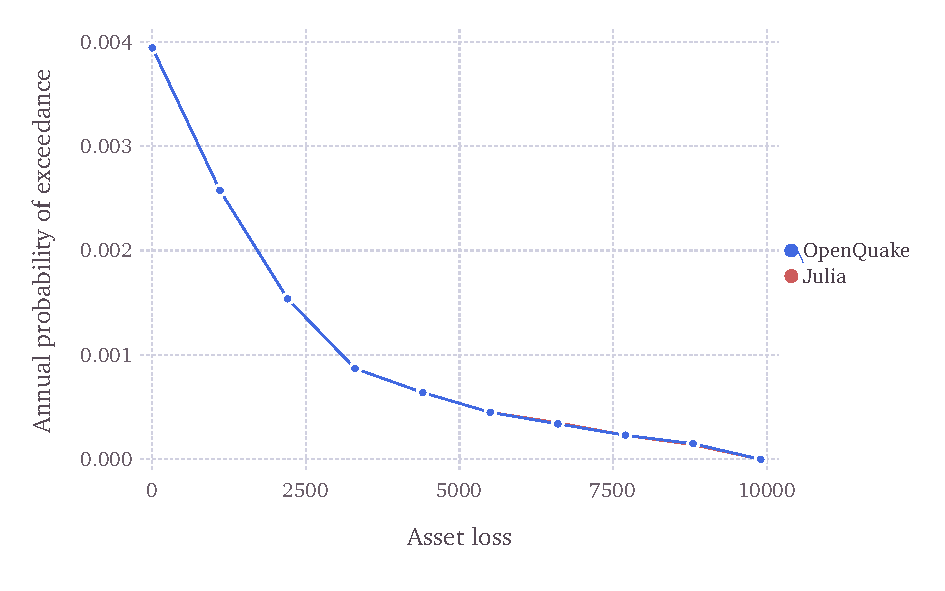
\includegraphics[width=12cm]{qareport/figures/fig-lc-ebr-1c}
\caption{Loss curve comparison for event based risk test case 1c}
\label{fig:lc-ebr-1c}
\end{figure}

The area under the annual loss exceedance curve gives the average annual loss.